\section{Approach}
\label{sec:approach}

%\begin{figure}[th]
%\centering
%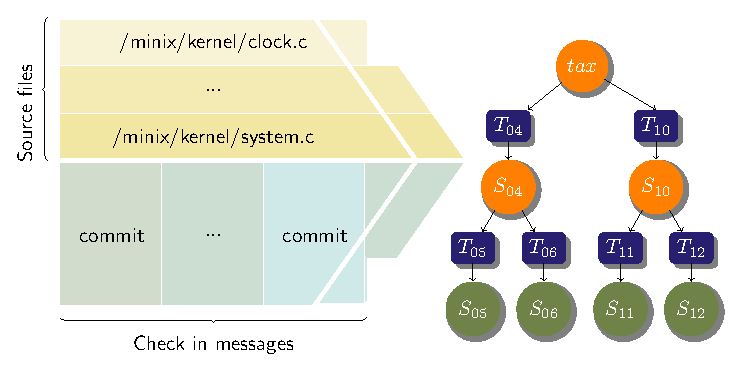
\includegraphics[width=0.8\columnwidth]{picture/framework.eps}
%\caption{ICQ Workflow. \textcircled{1}: data filtering phase; \textcircled{2}: cue discovery phase; 
%\textcircled{3}: model probing phase.}
%\label{fig:framework}
%\end{figure}

%The ICQ framework is illustrated in~\figref{fig:framework}.
We first define a set of linguistic features which are possible human artifacts and show 
how to neutralize them in a sentence. 
Then we present two simple methods to classify if a feature is extraneous in an NLR question.
Next we present several statistical metrics to compute the cueness score 
for a given extraneous feature using the information from a subset of questions that 
contain that feature.
%In \textit{data filtering} phase, it extracts from the dataset
%those problem instances that contain a given linguistic feature $f$. 
%In \textit{cue discovery} phase, it identifies the possible cues in this dataset. 
%Finally, in \textit{model probing} phase,
%it does two tests: ``accuracy test'' and ``distribution test''.
%Next we will discuss these phases in more details.

%\KZ{The workflow
%here evaluates the ``cueness'' of one specific linguistic feature $f$ of a
%given data set which consists of a training set and a test set.
%We first filter the training set and the test set respectively into two
%subsets of instances that carry the given linguistic feature. We then
%compare the label distribution of these two subsets (blue and red). If 
%there is substantial similarity, then the dataset is declared to be
%inflicted with the cue on $f$. 
%We can modify the test subset into a {\em neutral
%test} set $ST$
%by duplicating cases with underrepresented labels and effectively
%flattening the red distribution \KZ{use some notations here and in the fig
%for easy narration.} Now, suppose we have a model $M$,
%trained from the original training data, and we apply $M$ on the $ST$, to make
%predication results. If the label distribution of these results
%(green distribution) is again similar 
%with the original training data distribution (blue), we can conclude
%that model $M$ does exploit the feature $f$ in its inference and its
%accuracy maybe over-estimated.  Next we explore several
%shallow linguistic features which act as possible cues, and 
%give details on how the dataset and the model can be evaluated against
%these features.}

%
%ICQ can be broken down into the following phases: feature definition, 
%dataset filtering and evaluation, and model evaluation. With ICQ, we 
%discover whether the data have spurious cues, and whether a model is 
%sensitive to a particular linguistic feature during inference.

%WeWe evaluate the information leak in the datasets by statistical cues only. 
%First, we formulate  a number of NL reasoning tasks in a general form. 
%Then based on the cues associated with each label, 
%we design a number of metrics to measure the correlation between words
%and labels. Such correlation scores are called ``cue scores'' because they are 
%indicative of potential cue patterns. Afterwards, we aggregate the scores 
%using a number of simple statistical
%models to make the predictions. Finally, we show how to split a dataset into
%the easy and hard parts using the above fast predictions.

\subsection{Linguistic Features and Their Neutralization}
\label{sec:features}
\KZ{Add citation to each of the following feature (if previous work has used them
as bias feaure)?} 

In this work, we consider the following linguistic features: 
Word (unigram tokens in the input sentences), 
Typos, NER (named entity recognition), 
Tense (temporal order of events), Negation, 
Sentiment, and Overlap (words occurring both in the premise and 
the hypothesis). 
The above list is by no means exhaustive, but just a starting point for users 
who can come up with additional features that are relevant
to their task or domain. 

\subsubsection{Word} 
For a dataset $X$, we collect a set of all words 
$V$ that ever exist in $X$. 
%These 
%words can be word or cross-word that consists of a pair of
%unigrams, one from the premise and other from the hypothesis.
%the token pair between $p$ and $h$.
A word feature is defined as the existence of a word $w \in V$
in the hypothesis. 
%The cross-unigrams, such as  ``swimmer-sea'' in~\exref{exp:snli}, 
%represent the 
%relational unigrams in a dataset. 
%The ``swimmer-sea'' cross-unigram can be identified as a cue if it always appear in the instances with 
%one label, like entailment.
Because $V$ is generally very large, in practice, we may narrow it down
to words that are sufficiently popular in $X$. That is, we may disregard 
words that have low frequency in $X$.
To neutralize a word, we either delete it from the sentence, or replace it with one of its
synonyms, or simply an \textbf{UNK} token.
%the feature set to a smaller subset of words in $V$. Intuitively, 
%we want to pick those words that are strongly biased in
%the dataset, which means their occurrence is strongly
%correlated with some fixed label. There are a few choices for
%computing this bias. In this work, we choose to use the probabily
%of seeing word $w$ conditioned on label $l_i$:
%\begin{equation}
%   cp_{w,l} = p(w | l) = \frac{\#(w, l)}{\#(w)}
%\end{equation}
%where $\#(x)$ denotes the number of 
%instances in the dataset that contain $x$. \KZ{$w$ only in $h$ also?}
%
%The bias in a word is then computed as the mean square error over 
%$cp_{w,l}$:
%\begin{equation}
%bias(w) = \frac{1}{L} \sum_{l \in \mathcal{L}} (cp_{w,l} - \overline{cp_w})^2
%\end{equation}
%where $\overline{cp_w}$ is the average of $cp_{w,l}$ over all $l$ in $\mathcal{L}$.
%Words in $V$ with the top $bias(w)$ scores will be used as 
%word features.

%of $w$ with respect to label $l$ as
%%\KZ{Consider changing $\mathcal{F}$ to $\mathcal{B}$ to avoid confusion with $f$?}
%
%\begin{equation}
%    f_{\mathcal{F}}^{l} = f_{\mathcal{F}}(w, l),    
%\end{equation}
%%We call $f_{\mathcal{F}}^{(k,l)}$ \textit{cue metric}, 
%where $f_{\mathcal{F}}^{l}$ is a function which measures how much spurious information can be conveyed by token $w_k$ for a particular label $l$. 
%$\mathcal{F}$ is a set of cue metrics that we used for computing the \textit{cue score}. 

\subsubsection{Sentiment}
For each instance $x$, we compute its sentiment value as:
\begin{equation}
S(x) = \sgn(\sum_{w \in x} polar(w)),
\end{equation}
where $polar(w)$ is the sentiment polarity (-1, 0, or 1)
of $w$ determined by a look-up from a pretrained sentiment 
lexicon~\footnote{We use the spaCy NLP toolkit: \url{https://spacy.io}}.
We say $x$ has a positive/negative sentiment feature if $S(x)$ = 1 or -1 
respectively. Note that neutral is not a sentiment feature.
To neutralize the sentiment feature, we locate the sentiment word(s) in the
sentence, and replace them a word with opposite sentiment if there is one, otherwise
an UNK token.

\subsubsection{Tense}
We say that an instance $x$ has  
\textit{past}, \textit{present} or \textit{future} tense feature if $x$
carries one of these tenses, respectively, by the POS tag of the root verb
in $h$. We neutralize the tense feature but replace the root verb with
a different tense from the above three.

\subsubsection{Negation}
Previous work has observed that negative words (``no'', ``not'' or ``never'') 
may be indicative of a certain label in NLI tasks for some models.
The existence of a negation feature in $x$ is decided by dependency 
parsing. 
To neutralize negation, we delete the negative words in the sentence or
replace them with UNK token.

\subsubsection{Overlap}
In many models, substantial word-overlap between the premise and the
hypothesis sentences causes incorrect inference, 
even if they are unrelated~\cite{mccoy2019right}. 
%Very little word overlap causes a prediction
%of neutral instead of entailment.
We define that an overlap feature exists in $x$ if there's at least one word
(except for stop words) that occurs both in $p$ and $h$. 
To neutralize overlap, we replace the overlapping word $w$ in $h$ with its synonym that best
fit the language model.

\subsubsection{NER}
We define the NER feature as the existence of an instance of
PER, ORG, LOC, TIME, or CARDINAL in $h$.
We use the spaCy NER toolkit for this purpose. 
To neutralize NER, we a detected named entity with another
name entity of the same NER type in $h$, or UNK if there isn't any. 
%For example anchoring on named entities too strongly
%instead of understanding named entities and their
%impact on whether questions are duplicates. 

\subsubsection{Pronouns}
We define the Pronoun feature as the existence of one or more pronouns
in $h$. To neutralize this feature, we deploy coreference resolution
on the premise and hypothesis together as one sentence, and try to identify
a named entity or concept $e$ that the pronoun refers to. 
We then just replace the pronoun with $e$. If no such $e$ can be found
with high confidence, we will replace the pronoun with UNK.
 
\subsubsection{Typos}
We say an instance $x$ has typo feature if there exists at least one
typo in $h$.
We use a pretrained spelling model~\footnote{\url{https://github.com/barrust/pyspellchecker}} 
to detect all typos in a sentence. We don't distinguish the types of mispellings here. 
To neutralize the typo feature, we correct all the detected typos in $h$.
%We only pay attention to the features which have enough test data for model evaluation.
%In addition, we can analysis the credibility of test data through 
%the Kullback-Leibler (KL) Divergence. If a train dataset distribution is unbalance, 
%a similar distribution between train and T
%test can lead to insufficient test which test the cues mostly with a certain label. 

%As we mentioned in Example \ref{exp:roc}, multiple choice questions are each split into 
%two data instances with opposite labels (T or F), and the premises in these two
%instances are identical. Therefore, it is not useful to detect features within the premises
%alone. Consequently, for MCQ type of datasets, all the above features except for Overlap
%are only applied on the hypotheses.

\subsection{Extraneous Feature Classification}
Given a problem instance $(p, h, l)$, and a feature $f$ in $h$, we first neutralize $f$ in $h$
to obtain $h_{-f}$. We develop two classifiers. In the first one, we say $f$ is an extraneous
feature if $h$ and $h_{-f}$ are semantically close enough~(i.e., the semantic similarity~\footnote{We use SimCSE to compute sentence embedding: \url{https://github.com/princeton-nlp/SimCSE}} is larger than certain threshold), without considering the premise.
In the second one, we take the premise into account and 
apply an pre-trained NLI model~\footnote{\url{https://huggingface.co/symanto/mpnet-base-snli-mnli}} on $(p, h)$ and $(p, h_{-f})$, respectively. If the predicted distributions over \textit{entailment}, \textit{neutral} and \textit{contradiction} before and after 
feature neutralization are close enough~(i.e., the KL divergence is smaller than certain threshold), we deem $f$ as an extraneous feature.

\subsubsection{Human Annotation}
As described above, both semantic similarity based and NLI based classifiers rely on certain threshold value to determine whether a feature $f$ is
extraneous or not. In order to choose the threshold value, we conduct a human annotation procedure to collect groud-truth labels. For each dataset considered, we construct a dataset containing 200 questions in total sourced from original test set about ten features. 
In the original problems, there are two answer options in which only one is right. For each question, we also provide the corresponding feature $f$ that appears in one of its answer choice to the annotator. An example is shown as follows:

\begin{example}
\label{exp:roc2}
A story in ROCStory dataset, with ground-truth ending bolded.
\begin{description}
\item{Context:} Ala go to the park. There she saw a few of her friend. They challenged her to a game of Frisbee. Ala accepted the challenge .
\item{Ending 1:} \textbf{Ala won the game.}
\item{Ending 2:} Ala immediately left for work.
\item{Feature:} immediately
\end{description}
\end{example}

\begin{table}[th]
        \centering
        \scriptsize
        \begin{tabularx}{\columnwidth}{l|X}
                \toprule
                \textbf{Oper.} &\textbf{Instruction}\\
                \hline
                %\multirow{3}{*}{Word}
                Word&If a specific word as the feature was deleted from 
                vanilla choice, annotators should determine whether 
                the results of the questions with this word feature are reversed or not. \\
                \hline
                %\multirow{3}{*}{Sentiment}
                Sentiment
                &Given the sentiment of choice and the key tokens (polarity tokens with *), 
                annotators should determine whether the results of the questions 
                with these polarity features can reversed or not when the polarity are changed.\\
                \hline

                %\multirow{3}{*}{Tense} 
                Tense
                & We say that a choice has past, present or future tense feature.
                If the tense of a choice is changed to another tense, annotators should
                point out whether the results are changed. \\
                \hline
                %\multirow{3}{*}{Negation} 
                Negation
                & Similar with word feature, annotators are asked to determine the reasoning
                relationship is still valid without the negation tokens, like ``never''. 
                \\
                \hline
                %\multirow{3}{*}{Overlap} 
                Overlap
                & If the words in a choice are also appear in premise, annotators should 
                replace the words with their synonyms and determine whether this change 
                can influence question results. 
                \\
                \hline
                %\multirow{3}{*}{NER} 
                NER
                & If the entities are changed to other entities with the same entity types of
                vanilla choice, whether the reasoning relationship is valid or not. 
                \\
                \hline
                %\multirow{3}{*}{Pronouns} 
                Pronouns
                & Annotators should replace the pronouns in choices to their coreference nouns 
                and then judge whether the prediction results are changed or not. 
                \\
                \hline
                % \multirow{3}{*}{Typos} 
                Typos
                & Annotators are asked to retest on the questions with typos, if they still can
                choose the right choice, it means the typos can not influence the
                reasoning relationship. 
                \\ 

                \bottomrule
        \end{tabularx}
        \caption{Stress test operators considered in this paper. 
First line in each cell describes the operation, the remaining lines in
the cell give examples of how the operators work using input and output. 
r$\rightarrow$w indicates the operator turns a right choice into a wrong choice, while
w$\rightarrow$w indicates the operator turns a wrong choice into another wrong choice.} 
        \label{table:proxyop}
\end{table}


Human annotators are asked to adhere to the following protocol to determine the extraneousness label $e$ for each 
problem instance $(p,h,h_{-f},l)$: if $l=right$ and changing $h$ to $h_{-f}$ will flip $l$ to $wrong$ or $l=wrong$ and changing $h$ to $h_{-f}$ will flip $l$ to $right$, then $e$ should
be labled as $No$. Otherwise $e$ should be labled as $Yes$. In \exref{exp:roc2}, $e$ should be $Yes$.

\subsubsection{Searching for Threshold}
After the collection of human annotated extraneousness labels, we then proceed to tune the threshold value using a 5-fold cross validation
scheme. Assuming a list of $N$ problem instances $\{(p^i, h^i, h_{-f}^i, e^i)\}_{i=1}^{N}$ annotated with extraneousness labels $e^i\in \{Yes,No\}$, we first shuffle the list and evenly split
it into 5 non-overlapping subsets. For $k$-th fold, we treat the $k$-th subset as evaluation set and use the remaining four subsets as tuning set to search the threshold.


For semantic similarity based classifier, the initial threshold $\tau_{init}^k$ is calculated as the average cosine similarity between $h$ and $h_{-f}$ for all instances in the tuning set with $e=Yes$. 
Then we linearly decrease $\tau_{init}^k$ with a constant step size and find the threshold $\tau_{max}^k$ with highest tuning set accuracy. We obtain the final threshold $\tau_{sim}^*$ by taking the average of $\{\tau_{max}^k\}_{k=1}^5$.
The procedure is illustrated in Algorithm 1. $\tau_{sim}^*$ can then used to determine a feature $f$ is extraneousness or not in the future: if $M_{sim}(h, h_{-f}) \geq \tau_{sim}^*$, we regard $f$ as an extraneous feature.


\begin{algorithm}[th]
\caption{Searching the threshold using semantic similarity}
% \KwIn{$\{(p^i, h^i, h_{-f}^i)\}_{i=1}^{N}$, Pretrained sentence embedding model $\bm{M}$.}
% 1. 
\textbf{Input:} N labeled problem instances $I=\{(p^i, h^i, h_{-f}^i, e^i)\}_{i=1}^N$, step size $\alpha$, number of steps $T$, semantic similarity model $M_{sim}$.

1. Evenly split $I$ into 5 non-overlapping subsets $\{I_k\}_{k=1}^5$

2. \textbf{for} $k=1...5$:

    \quad \quad $\tau_{init}^k=Avg(M_{sim}(h^i, h_{-f}^i))$ s.t. $i\in \bm{I}_{-k}$ and $e^i=Yes$

    \quad \quad $\tau_{max}^k=\underset{\tau^k}{\arg\max}\ Accuracy(\tau_t^k, \bm{I}_{-k})$ where $\tau_t^k=\tau_{init}^k-\alpha*t$ and $0\leq t< T$

\textbf{Output:} $\tau_{sim}^*=\frac{1}{5}\sum_{k=1}^{5}\tau_{max}^{k}$
% \KwOut{Threshold value $\tau$}
\end{algorithm}

For NLI based classifier, the initial threshold $\tau_{init}$ is calculated as the average Kullback-Leibler divergence between NLI model's prediction distributions of 
$(p, h)$ and $(p, h_{-f})$ for all instances in the tuning set with $e=Yes$. We then linearly increase $\tau_{init}^k$ with a constant step size and find the threshold $\tau_{max}^k$ 
with highest tuning set accuracy. The final threshold $\tau_{NLI}^*$ is obtained by taking the average of $\{\tau_{max}^k\}_{k=1}^5$. 
The procedure is illustrated in Algorithm 2. $\tau_{NLI}^*$ is then used to determine if a feature $f$ is extraneousness or not: if $KLD(M_{NLI}(p,h), M_{NLI}(p,h_{-f})) \leq \tau_{NLI}^*$, we regard $f$ as an extraneous feature.



\begin{algorithm}[th]
\caption{Searching the threshold using NLI}
\textbf{Input:} N labeled problem instances $I=\{(p^i, h^i, h_{-f}^i, e^i)\}_{i=1}^N$, step size $\alpha$, number of steps $T$, NLI model $M_{NLI}$.

1. Evenly split $I$ into 5 non-overlapping subsets $\{I_k\}_{k=1}^5$

2. \textbf{for} $k=1...5$:

    \quad \quad $\tau_{init}^k=Avg(KLD(M_{NLI}(p^i,h^i), M_{NLI}(p^i,h_{-f}^i)))$ s.t. $i\in \bm{I}_{-k}$ and $e^i=Yes$

    \quad \quad $\tau_{max}^k=\underset{\tau^k}{\arg\max}\ Accuracy(\tau_t^k, \bm{I}_{-k})$ where $\tau_t^k=\tau_{init}^k+\alpha*t$ and $0\leq t< T$

\textbf{Output:} $\tau_{NLI}^*=\frac{1}{5}\sum_{k=1}^{5}\tau_{max}^{k}$
% \KwOut{Threshold value $\tau$}
\end{algorithm}

Instead of solely depending on $h$ and $h_{-f}$, NLI based classifier also incorporates the premise $p$, thus would intuitively
yield more accurate prediction. In our experiment, the 5-folds average evaluation set accuracies are 8x.x versus 83.4 for semantic similarily based and NLI based classifiers respectively, which echos with our 
assumption.

\subsection{Discovering Cues in Dataset}
\label{sec:evaldata}
Let $f$ be an extraneous feature, we compute the statistical 
correlation between $f$ and label $l \in \{true, false\}$, as $q^{(f,l)}$, in one of the 
following \textbf{four ways}. Note that the same feature $f$ may be 
extraneous in one instance but not in the other. \textbf{We only consider the instances
in which $f$ is extraneous}. \KZ{The frequecies might need to be recomputed!} 
Finally, we define the \textbf{cueness} score $q^f$ by computing the mean square error of
the correlation values across all possible labels.
%of $w$ with respect to label $l$ as
%%\KZ{Consider changing $\mathcal{F}$ to $\mathcal{B}$ to avoid confusion with $f$?}
%
%\begin{equation}
%    f_{\mathcal{F}}^{l} = f_{\mathcal{F}}(w, l),    
%\end{equation}
%%We call $f_{\mathcal{F}}^{(k,l)}$ \textit{cue metric}, 
%where $f_{\mathcal{F}}^{l}$ is a function which measures how much spurious information can be conveyed by token $w_k$ for a particular label $l$. 
%$\mathcal{F}$ is a set of cue metrics that we used for computing the \textit{cue score}. 
%Let $\LL' = \LL - \{l\}$ and we define
%\begin{equation}
%    \#(f, \LL') = \sum_{l' \in \LL'} \#(f, l').
%\end{equation}
%Think of $v_f=[\#(f, l), \#(f, \LL')]$ and $v_l = [(\#(l), \#\LL')]$ 
%are two vectors on a 2D plane.
%Intuitively, if $v_f$ and $v_l$ are co-linear, $f$ leaks no spurious information.
%Otherwise, $f$ is suspected to be a spurious cue as it tends to appear
%more with a specific label $l$.
%

\subsubsection{Frequency(Freq)}
The most simple but straight measurement is the co-occur of the
words and labels, where $\#()$ means naive counting.
\begin{equation}
    q_{Freq}^{(f,l)} = \#(f, l)
\end{equation}

\subsubsection{Conditional Probability(CP)}
The distribution of a dataset based on label may not always balance.
So we also try conditional probability as a measurement of correlation.
\begin{equation}
    q_{CP}^{(f,l)} = \frac{\#(f, l)}{\#(f)}
\end{equation}

\subsubsection{Point-wise Mutual Information (PMI)}
PMI is a widely used method for association measurement in information theory and statistics.
We estimate the probability:
\begin{equation}
p(l) = \frac{\#(l)}{\#(\mathcal{L})}, p(l|f) = \frac{\#(f, l)}{\#(f)},
\end{equation}
where $\#(\mathcal{L}) = \sum_{l\in \mathcal{L}} \#(l)$.
The PMI score of token $f$ with respect to label $l$ is
\begin{equation}
    q_{PMI}^{(f,l)} = \log \frac{p(l|f)}{p(l)}
\end{equation}

\subsubsection{Local Mutual Information (LMI)}
Considering the frequency of tokens can influence models with different weight and inspired
by \cite{schuster2019towards},
we estimate the probability by
\begin{equation}
    p(f, l) = \#(f, l) / \sum_{i=1}^{|\mathcal{N}|}\#(f_i).
\end{equation}
The LMI of feature $f$ with respect to label $l$ is:
\begin{equation}
    q_{LMI}^{(f,l)} = p(f, l)\log \frac{p(l|f)}{p(l)}.
\end{equation}

\subsubsection{Cueness score}
%Given the features $F$,
%Once we have defined the linguistic features, we can build a data filter for
%each feature values. A filter takes a dataset and returns
%a subset of instances associated with that feature value. For example,
%there is a filter for the word ``like''; there is a filter for ``PER'' entity;
%and there is filter for ``negative'' sentiment, etc. 
%
%For each feature $f$, we apply its filter to both the training data and test data
%of $X$, denoted as $R$ and $S$ in \figref{fig:framework},
%resulting in $R_f$ and $S_f$. 
%Only those features that appear both in the training and test data
%are qualified as possible cues for a dataset.
%Let $y_i$ be the number of instances with label $l_i$ in the filtered
%dataset, then we can compute the bias of the label distribution for a filtered
%set as the mean squared error (MSE):

\begin{equation}
q_{MSE}^{f} = \frac{1}{|\LL|} \sum_{l \in \LL}\left(q^{(f,l)} - \frac{\sum_{l \in \LL} q^{(f,l)}}{|\LL|}\right)^2
\end{equation}
The larger $q_{MSE}^f$, the more likely feature $f$ is a spurious cue in this dataset, which means
feature $f$ is distributed unevenly toward one of the labels. 
We are now able to rank all the features in an NLR dataset (the training set in particular)
by the cueness score. The top features on that list are the spurious cues in that dataset.
%Furthermore, if the filtered training set and the filtered test set are biased similarly,
%the Jensen-Shannon Divergence~\cite{lin1991divergence} between them is small:
%\begin{equation}
%jsd(R_f, S_f) = \frac{1}{2}\left (R_f\parallel M  \right )+\frac{1}{2}\left (S_f\parallel M  \right ), 
%\end{equation}
%where $M= \frac{1}{2}\left (R_f+S_f \right )$. 
%%\KZ{Complete the above formula.} 
%Finally, we define a cueness score as
%\begin{equation}
%cue(f, X) = \frac{mse(R_f)}{\exp(jsd(R_f), S_f))}
%\end{equation} 
%which represents how much a dataset $X$ is biased against a feature
%$f$. 
%\KZ{Add a comparison between this cue function and other possible cue functions
%such as PMI in eval. By computing the distance between the ranking induced by
%the cueness and the rankings by the four models $\Delta$.}
%
%\subsection{Probing Bias in Model}
%\label{sec:evalmodel}
%
%Suppose we already know that a dataset $X$ is infected with a cue $f$ from previous
%test in \secref{sec:evaldata}.
%However, just because the dataset is infected with a cue doesn't mean
%the model trained from this dataset necessarily exploits that cue.
%Here we propose a simple method to probe any model instance trained from the
%given biased dataset~\footnote{Models trained from any other 
%datasets compatible in format with $X$ can also be used to probe its potential
%bias on the same cue.} to see if it actually takes advantage of that cue $f$
%and by how much.
%
%We can do that through two simple tests: 
%{\em accuracy test} and {\em distribution test}.
%In accuracy test, we simply assess the prediction accuracies of the model
%$M$ on the filtered test set and on the remaining test data, and call them
%$acc(S_f)$ and $acc(S_{nf})$, respectively. The accuracy test says that if the difference
%between these two accuracies, i.e, $\Delta=acc(S_f) - acc(S_{nf})$ is greater 0, then the
%model is considered to be biased and to have exploited this cue. 
%The value of $\Delta$ measures the extent of the bias.
% 
%Distribution test is a visual test. We first create a ``stress data set'' $\overline{S_f}$
%by ``flattening'' the label distribution in $S_f$.  
%We achieve that by replicating random instances from all labels 
%except the most popular label in the filtered test
%set and adding them back into the set. 
%The repetition augmentation procedure stops when 
%the feature distribution based on each label is balanced.
%This way we have effectively removed the bias 
%in the filtered test set and presumably 
%posed a challenge to the model. 
%Next we apply the same model on the stress test set 
%to get prediction results. 
%We compare the label distribution of the prediction results on 
%the stress test set with the label distribution of 
%the filtered training data.
%The idea is, if the filtered training data contains a cue, 
%its label distribution will be skewed toward a particular label.
%If the model exploits this cue, it will prefer to predict
%that label as much as possible, even amplifying the skewness
%of the distribution, despite that the input test set has been
%neutralized already. We hope to witness such an amplification
%in the output distribution to capture
%the weakness in the model.
%
%%If the two distributions are similar enough, 
%%we deem the model biased toward that feature and not robust enough.
%%This similarily can be displayed visually. 
%The above two tests are related but not equivalent
%and their outcome complement and reinforce each other. 
%
%but don't provide new method for data augmentation. 
%We require a more fair dataset to test if a model is sensitive to a feature. 
%The filtered test dataset of a feature in \figref{fig:framework} (red) is unbalanced among 
%labels. The number of cases for each label can be denoted as $c_{ent}, c_{neu}, c_{con}$~(in 
%SNLI task). If any of these number is smaller than a threshold $\sigma$, 
%we won't consider to test this feature, because
% this feature is not well supported by enough data. 
%%If the smallest number of samples among different labels is lower than 
%%a threshold $\sigma$, we won't consider to test this feature. Because
%% this feature is not well supported by enough data. 
%The smallest number can be denoted as $c_{min}=min(c_{ent}, c_{neu}, c_{con})$.
%To make the result more intuitive and fair, 
%we flatten the distribution by removing $c_{l} - c_{min}$ cases from 
%the filtered cases with label $l$ 
%resulting in the orange ``stress test'' 
%in \figref{fig:framework}. 
%Then we test the model on this stress test. 
%The similarity between prediction result (green) and 
%training data distribution (blue) on a feature indicates how the model 
%is influenced by the appearance of this feature in training data. 

%It is insufficient for testing if the filtered test data size is quite small or samples on 
%some label is rare which bellow a threshold $\sigma$. 
%Thought we can't generate cases for feature, we can point out what kind of 
%test samples should be augmented. 
%The similarity is 
%calculated by Kullback-Leibler (KL) Divergence.

\subsection{Testing for Biases in the Model}
Our test goes through two phases. In phase one, we test the targeted model trained on an NLR dataset. 
In phase two, if this model is fine-tuned on top of a pretrained language model such as
BERT or RoBerTa, we will test the original PLM by prompting. Next we describe these two phases
in turn.

\subsubsection{Test task-specific model}
For every question in the test set, we first detect all the extraneous features. Then for each
extraneous feature, we generate a neutralized version of the same question. We then apply the model
on both the original question and the feature-neutral question. If the model predicts different labels,
then the model is said to be sensitive to this extraneous feature in this question.
After all questions and all extraneous features are tested, we can compute the model's sensitivity
to each extraneous feature statistically. In other words, the model will be associated with a ranked
list of extraneous features. Can we thus compare the lists of different models trained from the
same training data and see which model is weaker and due to what features.
 
\subsubsection{Test the PLM}
\KZ{Roy, pls complete this part?}

